
% ========================================================================== %
%                                                                            %
%                                 PREAMBLE                                   %
%                                                                            %
% ========================================================================== %

% Define document class
\documentclass[a4paper,11pt,titlepage]{article}
\usepackage[onehalfspacing]{setspace}

% Define geometry/positioning of of text
\usepackage[paper=a4paper,left=20mm,right=20mm,top=30mm,bottom =30mm]{geometry}

% Grammatic packages
\usepackage[ngerman,english]{babel}
\usepackage[utf8]{inputenc}
\usepackage[T1]{fontenc}
\usepackage[font=small, textfont=it, labelfont=it,bf, format=hang]{caption}

% Create headers
\usepackage{fancyhdr}
\pagestyle{fancy}
\headheight 14pt
\renewcommand{\headrulewidth}{0.4pt}
\renewcommand{\footrulewidth}{0.4pt}

% To comment text blocks
\usepackage{comment}  % --> \begin{comment} ... \end{comment}

% Packages affecting text, pictures and tables
\usepackage{multicol} 
\usepackage{graphicx}
\usepackage{caption}
\usepackage{float}
\usepackage{array}
\usepackage{booktabs}
\usepackage{xcolor}
\usepackage[section]{placeins} 	% pictures won't jump into other sections!
\usepackage{wrapfig} % Text aside pictures
\usepackage{rotating} % Allows rotated picturses AND captions!
\usepackage{pdfpages}

% Mathematical modus packages
\usepackage{mathptmx}
\usepackage{amsmath}

% Packages for bibliography and references
\usepackage[authoryear]{natbib}
\usepackage[colorlinks]{hyperref}
\hypersetup{colorlinks,
linkcolor={black},
citecolor={blue!55!black},
urlcolor={blue!70!black}}
\usepackage{apalike}
\usepackage{chngcntr}

%Package for text symbols
\usepackage{txfonts}
\usepackage{enumitem}
% ========================================================================== %
%                                                                            %
%                           DOCUMENT STARTS HERE                             %
%                                                                            %
% ========================================================================== %

\begin{document}

% ========================================================================== %
%                                                                            %
%                              DEFINE TITLE PAGE                             %
%                                                                            %
% ========================================================================== %

\begin{figure}
\centering
\vspace{-1.5cm}
\hspace{-1cm}
\begin{minipage}{.3\textwidth}
  \centering
  
\includegraphics[width=\linewidth]{pictures/eth_logo_kurz_pos.eps}
  \label{fig:ETHlogo}
\end{minipage}
\vspace{1.5cm}
\hspace{5cm}
\begin{minipage}{.2\textwidth}
  \centering
  
\includegraphics[width=\linewidth]{pictures/logo_D_ERDW_pfade.eps}
  \label{fig:LogoERDW}
\end{minipage}
\end{figure}


\title{\huge{Direct Dating of Skarn-Mineralization at Bingham Canyon Porphyry-Cu-Au Deposit, Utah, using Garnet U-Pb and Sm-Nd Isotopes.}}
\author{\LARGE{{MSc Project Proposal}
\vspace{10pt}}
\\
Jari Klingler \\ \\\vspace{20pt}  \and 
Supervisor: Dr. Albrecht Quadt Wykradt-Hüchtenbruck, ETH Zürich, \\ Institute for Geochemistry and Petrology \vspace{2pt}\and Co-Supervisor: Dr. Dr. Oscar Laurent, ETH Zürich, IInstitute for Geochemistry and Petrology \vspace{2pt}\and Co-Supervisor: Prof. Dr. Cyril Chelle-Michou, ETH Zürich, Institute for Geochemistry \\ and Petrology
\vspace{40pt}
\\Department of Earth Sciences, ETH Zürich}
\date{Zürich, \today}

\maketitle

\newpage

% ========================================================================== %
%                                                                            %
%                         DECLARATION OF ORIGINALITY                         %
%                                                                            %
% ========================================================================== %

% ========================================================================== %
%\begin{comment}

\thispagestyle{empty} 
\vspace{0.5cm}
\begin{center}
\LARGE{\textbf{Declaration of Originality}} \\
\end{center}
\vspace{1.5cm}
\noindent I hereby confirm that I am the sole author of the written work here enclosed and that I have compiled it in my own words. Parts excepted are corrections of form and content by the supervisors. \\
\\
\\
\noindent \textbf{Title of work:}\\
\\
\textit{Direct Dating of Skarn-Mineralization at Bingham Canyon Porphyry-Cu-Au Deposit, Utah, using Garnet U-Pb and Sm-Nd Isotopes}
\\ \\
\noindent \textbf{Authored by:}\\
\\
Jari Klingler
\\
\\
\\
\noindent With my signature I confirm that:\\
\begin{itemize}
    \item I have committed none of the forms of plagiarism described in the 'Citation etiquette' information sheet.
    \item I have documented all methods, data and processes truthfully.
    \item I have not manipulated any data. 
    \item I have mentioned all persons who were significant facilitators of the work. 
\end{itemize}
\vspace{1.5cm}
 
I am aware that the work may be screened electronically for plagiarism. \\
\vspace{0.5cm}

\begin{center}
    \textbf{Place, date:}      Zurich, \today\\
\end{center}
\vspace{0.01cm}
\begin{center}
\textbf{Signature: }$\rule{4cm}{0.15mm}$\\
\end{center}

%\end{comment}

%\begin{comment}
%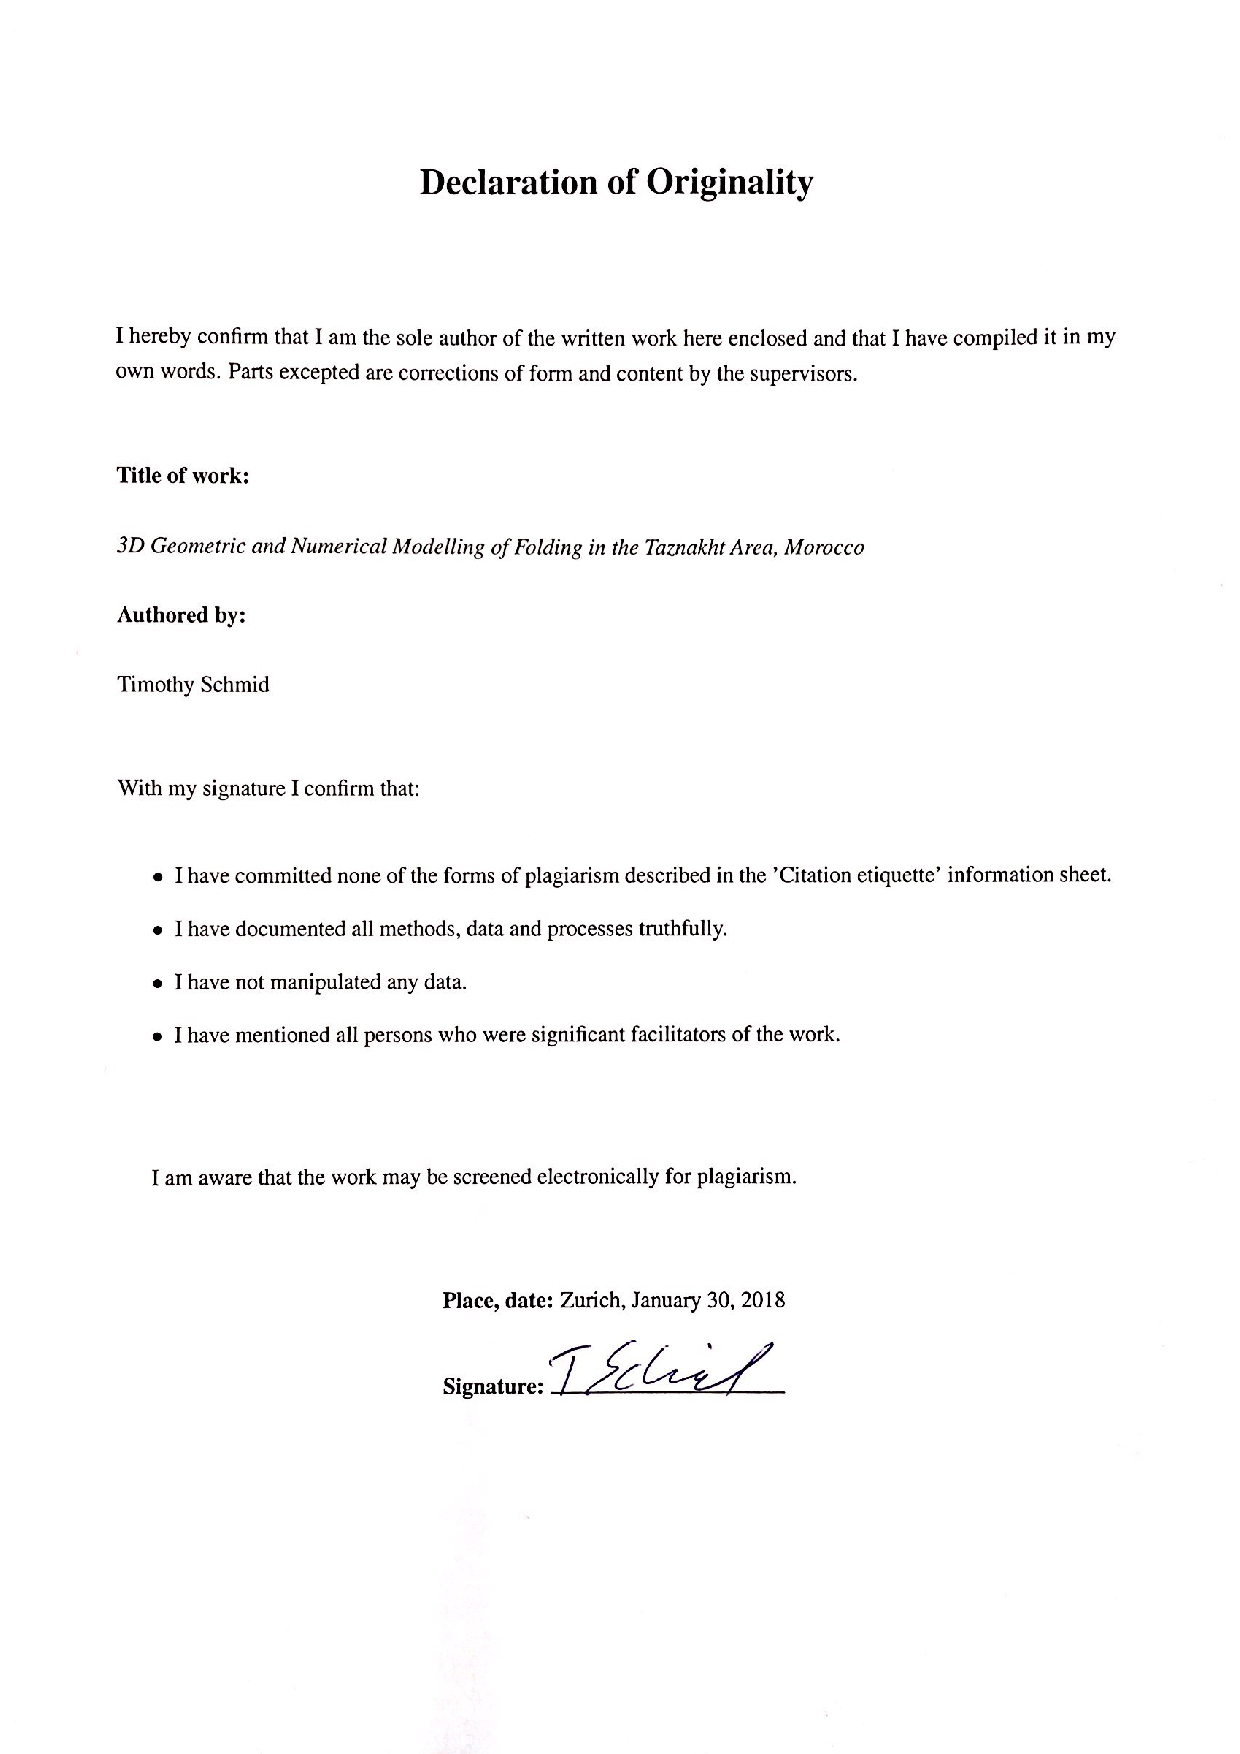
\includepdf[pages={1}]{Declaration.pdf}
%\end{comment}

% ========================================================================== %


% ========================================================================== %
%                                                                            %
%                                 ABSTRACT                                   %
%                                                                            %
% ========================================================================== %

\section{Abstract}

% ========================================================================== %
%                                                                            %
%                              TABLE OF CONTENTS                             %
%                                                                            %
% ========================================================================== %

\newpage
\tableofcontents
\thispagestyle{empty}

\newpage


% ========================================================================== %
%                                                                            %
%                                 INTRODUCTION                               %
%                                                                            %
% ========================================================================== %


\section{Introduction}

The Bingham Canyon Open Pit Copper mine (Rio Tinto Kennecott) houses one one the world's largest Cu-Au-Mo porphyry deposits. It is located about 35 km southwest of Salt Lake city, Utah, USA, in the central Oquirrh Mountain range. Rio Tinto Kennecott accounts for almost 11 per cent of the US’s annual copper production and is one of the largest copper producers in the country \citep{Tinto2017}.
\\The mine has been in use since 1906 and has an annual yield of over 405 kt Cu, at an average ore grade of 0.74\%, 12 t Au at 0.4458 g/t, 15kt Mo averaging at 0.035\% and 100 t Ag with 3.29 g/t \citep{Porter2012,Tinto2017}. Rio Tinto Kennecott’s mined copper production was 3 per cent lower than 2016, with lower grades partially offset by higher mill throughput. The operation produced 126 thousand tonnes of refined copper, 204 thousand ounces of refined gold, and five thousand tonnes of molybdenum in 2017 \citep{Tinto2017}, with skarns contributing about 10\% of the mined bulk metal resources with exceedingly high ore grades at 20 Mt: 3.65\% Cu, 1.62 g/t Au and 20.95 g/t Ag \citep{Krahulec2010,Jowitt2013}. 
\\
\\ Skarns typically occur together with many porphyry deposits (SILLITOE2010). Skarn deposits are commonly formed in complex, mixed host rocks, including carbonate-bearing sediments, volcanic and plutonic rocks through intrusion events of prophyries \citep{Einaudi1982}. Calc-silicate mineral assemblages developed in close proximity of intrusions within sediment units by metasomatism of silty limestones and carbonaceous sand- and siltstones, leading to the formation of skarns  and diopside hornfels respectively \citep{Atkinson1978a}.
\\
\\ SOMETHING ABOUT GEOCHRONOLOGY


%========================================================================== %
%                                                                            %
%                 BACKGROUND AND RESULTS TO DATE         %
%                                                                            %
% ========================================================================== %

\vspace*{10pt}
\section{Background \& Results to Date}

Skarns and the ores that they host, have established themselves as a valuable resource. Previous studies on skarns of the Bingham mining district have been accomplished with a focus on the stratigraphy, mineralogy, structural geology and chemical evolution of the Carr Fork area, which hosts high-grade gold and polymetallic mineralization in the contact aureole of the Bingham porphyry deposit \citep{Hunt1924, Lindgren1924, Winchell1924, Hansen1961, Atkinson1978a,Reid1978,Starkins1983,Cameron1987,Schloeglova2018}. 
\\
\\ Further, many radiometric geochronological studies have been conducted in the Bingham minin district to determine the age of intrusions, mineralization stages, the sequence and duration of hydrothermal activity \citep{Armstrong1970,Chesley1997,Deino1997,Kendrick2001b,Moore1973,Moore1971,Moore1968,Parry1997,Parry2001, Warnaars1978,Martinek2009}. The results of earlier studies show similar results to more recent ones, but with larger uncertainties.
\\
\\ Garnet contains U and minor Pb and has a high closure temperature for the U-Pb isotope system \citep{Mezger1989}, making it a viable choice for geochronological analysis \citep{Burton1992,Vance1993,Burton1995,Jung2003}. Dating the garnet of skarns may potentiall provide insights and constraints on the and history of magma emplacement and hydrothermal processes \citep{Heaman2001,Seman2017,Deng2017,Yang2018,Wafforn2018}.
\\ In U-poor metamorphic garnets, the presence of U-rich mineral inclusions, such as uraninite, zircon, monazite and allanite, makes analyses very challenging \citep{Dewolf1996,Vance1998,Lima2012}, and the use of garnet U-Pb as a geochronological method has been neglected, although it has been successful before \citep{Mezger1989}. Further, the Nd initial isotope ratios can vary strongly, complicating Sm-Nd dating as well \citep{Jamtveit1994}.
\\ Very recent studies by \citet{Deng2017} and \citet{Wafforn2018} have shown that U-Pb geochronology of garnets in skarns has been consistent with zircon U-Pb dates of the respective ore-related intrusions, confirming suitability and reliability for accurate dating for certain garnet-bearing magmatic rocks and hydrothermal alterations. 


% ========================================================================== %
%                                                                            %
%                    			              Goal									  %
%                                                                            %
% ========================================================================== %

\vspace*{10pt}
\section{Research Goals}

The aim of the study is to test a potential geological application, whether the U-Pb and Sm-Nd garnet dating can yield more accurate and reliable ages on porphyry-related mineralization, because so far it is generally only indirectly bracketed using zircon dating from the associated porphyry intrusions. In the Bingham Canyon porphyry-related Cu-Mo-Au deposit samples it is possible to texturally relate a specific generation of garnet to the sulfide ore, so that if we date the garnet, we directly date the mineralization. Multiple geochronology projects have been completed in previous studies for this region, but none have been done for the garnet mineralization within the skarns.
\\
\\
Further, we want to investigate whether we would be able to identify temporal differences between the deep and shallower skarn units, based on TIMS U-Pb garnet dating. The two systems are quite different relative to mineralization. The deep skarn unit is barren and could be therefore representative of the early skarn formation, while the shallower skarns that host the Cu-Au mineralization are possibly younger.

% ========================================================================== %
%                                                                            %
%                 						Geology         							%
%                                                                            %
% ========================================================================== %

\vspace*{10pt}
\section{Geology}

\subsection{Tectonic Setting}
The Bingham Canyon mine is located in the central Oquirrh Mountain range, north-central Utah, USA. It is located at the eastern side of the Great Basin and are separated from the Colorado Plateau by the north-south striking Wasatch Fault.
\\
\\ FIGURE >>> GEOLOGICAL MAP
\\\noindent The mountain range has been an area with an active tectonic past, including a cratonic margin that has been active since Archaean time, the east-west striking Uinta Axis and the overlap between the eastern boundary of the Basin and Range extensional terrain to the west and the Cordilleran fold and thrust belt to the east \citep{Babcock1995}. 
The Oquirrh Mountain region was a passive continental margin and experiencing subsidence and shelf sedimentation of thinly interbedded carbonates and siliclastic sediments during the Paleozoic until the late Carboniferous . Following, subsidence of the shallow water carbonates and rapid deposition of siliclastic rocks occurred within the northwest-trending Oquirrh Basin. During the early Permian, there was a return to a passive margin sedimentation \citep{Babcock1995,Presnell1991}.
\\There were two defining Mesozoic orogenies with complex deformation history that affected the region: the Mid Jurassic Elko Orogeny (170 - 150 Ma) and the Late Cretaceous Sevier Orogeny (110 - 65 Ma). During these periods of east-west oriented crustal shortening the series of northwest-trending folds south of Bingham Canyon and northeast-trending folds north of Bingham Canyon were formed, including several major thrusts and complex faulting and folding near the Cu-Mo-Au ore deposit \citep{Babcock1995,Presnell1997,Gunter1997}.
\\During the Cenozoic, a  extensional period with igneous activity developed. During the Eocene, intrusive and volcanic activity evolved during a minor extensional period, with associated emplacement of intrusions, dikes and fissures along the Uinta Axis, forming the west-oriented Wasatch igneous belt, resulting in the formation of the Bingham Canyon porphyry copper deposit \citep{Waite1997}.
\\The alignment of intrusions with the east-west orientation of the Uinta Axis, shows evidence for a northeast-directed structural control related to extension \citep{Presnell1997}. Some magmatic stocks and dikes reached the surface and formed a composite volcano during the Eocene, of which some parts are still preserved within the eastern flanks of the Oquirrh Mountain range \citep{Waite1997}.
\\The extension period continued with major Miocene to Recent Basin and Range extension, where faulting opened up Salt Lake valley more north-south-trending basins along major listric normal faults, accompanied by the eastward tilting of the Bingham Canyon deposit by 10-20 degrees \citep{John1989,Melker1997}.

\subsection{Geological Setting}

The mining district is primarily focused on the Bingham Stock, which contains most of the porphyry deposit. The stock consists of Equigranular Monzonite (EM), which was intruded by a dike-like body of Quartz Monzonite Prophyry (QMP), sills of Latite Porphyry (LP) and thinner dikes of Quartz Latite Porphyry (QLP) and a few smaller units \citep{Porter2012}.

\subsubsection{Sedimentary Rocks}

The open sedimentary layers within the district are comprised of parts of the Butterfield Peaks Formation (BPF) and the overlying Bingham Mine Formation (BMF) of the Oquirrh Group (Pennsylvanian). Both formations mainly include quartzites and lesser limestones, calcareous siltstones and sandstones \citep{Lanier1978}.
\\The BPF is the oldest geological unit within the mining area with emergence in the southern to south-western regions of the mine. The rocks within this formation consist of feldspathic orthoquartzite and calcareous quartzite, with interbedding of calcareous sandstones and arenaceous limestone, called the Sub-Jordan beds, and with a few exceptions not ore bearing \citep{Lanier1978}.
\\Overlying the BPF is the Bingham Mine Formation, which ha a lower and upper member. The lower member consist of two cherty limestone beds, the Jordan and Commercial Limestone beds. They are stratigraphic marker beds in the BMF and the most important sedimentary ore host in the district. They are the host for Cu-Au skarns in the northwestern area of the mine and Pb-Zn-Ag deposits at the eastern margin of the porphyry deposit \citep{Lanier1978}; MARTINEK2009).
\\The upper member of the BMF mostly consists of quartzite, and in comparison to the lower member, considerably fewer limestone and sandstone beds \citep{Lanier1978}.
\\The thinly bedded silty limestones and sandstones of the Curry Peak Formation and the interbedded quartzites and sandstones of the Freeman Peak formation overlie the BMF in the North. Ontop of these units lies the calcerous sandstone of the Diamond Creek Formation, which is superimposed by the cherty, phosphatic dolomite and dolomitic sandstone of the Permian Park City Formation. These units are the host of two Au deposits at Barneys Canyon and Melco, outside the the Bingham Canyon Mine \citep{Babcock1995}.
\\
\\>>>> FIGURE Stratigraphy

\subsubsection{Igneous Rocks}

The Bingham and Last Chance stock along with nearby plutons in the Butterfield Canyon are similar in texture, composition and are connected by dikes. This indicates that rock masses that have been separated surficially can converge at depth, forming a single stock. The intrusions generally are discordant with their irregular outline. The Bingham stock is an epizonal intrusion with a maximum cover thickness of 2300 $\pm$ 300 m \citep{Lanier1978}.
\\
\\ >> FIGURE CROSSECTION PORPHYRY DEPOSIT (redmond, einaudi 2010?)
\\
The following section gives a short description of the individual intrusive rock units, emplaced in the Bingham Canyon porphyry deposit, not including more peripheral units, such as the hybrid quartz monzonite porphyry or the porphyritic quartz monzonite, in sequence from oldest to youngest. 
\\
\\\underline{Equigranular Monzonite (EM)}
\\The EM is the oldest phase and most abundant igneous rock type in the Bingham Stock and an important sulfide host rock for the porphyry copper deposit. The intrusion happened pre-mineralization in one intrusive phase, which connects the north-eastern Bingham Stock and the south-eastern Last Chance Stock \citep{Parry2001}.
\\ The Last Chance Stock is located directly south of the Bingham Canyon open pit and appears to be unaltered, whereas the Bingham Stock, which is within the pit, shows high propylitic alteration and hosting a substantial amount of the Cu deposit \citep{Babcock1995}.
\\ The mineral assemblage of the unaltered monzonite consists of plagioclase (33\%), K-feldspar (30\%), quartz (7\%), which lies on the border between a quartz monzonite and a monzonite. Further it contains augite (11\%), uralitic amphibole (7\%), biotite (8\%), magnetite (2\%) and other accessory minerals \citep{Lanier1978}.
\\
\\\underline{Quartz Monzonite Porphyry (QMP)}
\\ The major intrusive phase into the Bingham Stock is the QMP. The intrusion formed a northeast-southwest striking and northwest dipping dike which concurs with the centre of mineralization in the mining district \citep{Lanier1978}. It contains the highest copper and gold grades in porphyry-hosted ore \citep{Redmond2010a}.
\\ Most of this rock type is overprinted by silicification and sericitic alteration. Portions, which do not show the overprint, show a significant amount of argillized feldspar (50\% phenocrysts) and phlogopitized amphibole in an aphanitic groundmass . The mineral assemblage of the unaltered rock type is estimated to be plagioclase (32\%), orthoclase (32\%), quatz (23\%) and mafic and accessory minerals (14\%), which classifies as a hornblende-biotite quartz monzonite \citep{Lanier1978}.
\\
\\\underline{Latite Porphyry (LP)}
\\ A series of northeast-trending sills and dikes which pass through the northwest margin of the Bingham Stock, including the Main Hill dike, the Starless dike and Fortuna sill, are formed by the LP. These dikes have also been found in the Carr Fork area and show textural and compositional variability, which are related to cooling environment and emplacement of the dikes during different magmatic surges \citep{Lanier1978}.
\\ The mineral assemblage of the LP resembles a composition of an unaltered amphibole-biotite quartz latite. Half to two thirds of the rock is comprised of a fine-grained quartz and orthoclase grains. Plagioclase is the main constituent of the phenocryst assemblage, with minor orthoclase, biotite, amphibole and small and rare, partially resorbed quatz grains \citep{Lanier1978}.
\\
\\\underline{Biotite Porphyry (BP)}
\\ The BP cuts through QMP and LP and ist truncated by the Quartz Latite Porphyry Breccia (QLPbx) and occurs as xenolith within the brecciated unit. Due to the increased content of biotite as phenocrysts (12-15\%) and within the groundmass, this porphyry appears much darker than the others and can contain smaller angular fragments of QMP and LP. Locally, BP hosts high-grade copper-gold ore and quartz veins and is potassically altered. The grades can vary and decrease rapidly, but likely not the result of overprinting by later fluid interaction from a younger porphyry intrusion \citep{Redmond2010a}.
\\
\\\underline{Quartz Latite Porphyry Breccia (QLPbx):}
\\ The QLPbx cuts through QMP, LP and BP and is the only intrusion that contains abundant wall-rock xenoliths, which make up 20-50 vol percent of the rock. QMP and LP fragments are contained within the breccia and contain many generations of truncated quartz veins with bornite-chalcopyrite, which indicates the emplacement of QLPbx after vein formation and sulfide deposition in LP. QLPbx has a aplitic-textured K-feldspar, quartz and biotite groundmass with numerous irregular vesicles (2-5\%) and phenocrysts of plagioclase and K-feldspar (11-17\%), biotite, biotitized hornblende and rare quartz eyes \citep{Redmond2010a}.
\\
\\\underline{Quartz Latite Porphyry (QLP)}
\\ As the youngest intrusion, the QLP forms narrow dikes. At the bottom of the mine, smaller apophyses are less altered, mineralized and fractured than the wall-rock itself \citep{Lanier1978,Stringham1953}. 
\\ The composition of unaltered phenocrysts shows, large feldspars (25\%), quartz (8\%) and biotite (6\%) with a groundmass consisting of the same composition \citep{Lanier1978}. QLP has a composition of fewer phenocrysts and increasing vol percentage of groundmass in comparison with the older porphyry intrusions \citep{Redmond2010a}.Further, QLP is a host for late-stage chalcopyrite and pyrite mineralization \citep{Babcock1995}. 
\\
\\>>FIGURE INTRUSIVE ROCKS

\subsubsection{Structures}

The development of structural elements within the region acted as controls on the emplacement of intrusions and are further important for the distribution pattern and mineralization within the northern Oquirrh Mountains \citep{James1961}. Major faults in the district are steeply dipping, north northeast-striking faults forming in the Mesozoic orogenous period with reactivation as normal faults during the Basin and Range extension in the Eocene \citep{Farmin1933,Tooker1971,Atkinson1978a,Redmond2010a}. The folds which were developed during the Mesozoic orogenies and the northeast-trending Cenozoic stuctures controlled the emplacement of the intrusions within the Bingham Canyon District \citep{Presnell1997}.
\\
\\\underline{Folds}
\\ The folds at Bingham Canyon are in accord with the regional patterns in the southern part of the Oquirrh Mountain range and shows large, generally open and northwest-trending arcuate anticlines and synclines \citep{Boutwell1905,Gilluly1932}.
\\ The Bingham Syncline and the Copperton Anticline represent the two major fold sets occurring in the Bingham Mining District, separated by the southwest-dipping Midas Thrust fault \citep{Keith1905}.
\\ The Bingham Syncline is the dominant fold in the mining district and is a broad, open fold below the mouth of Carr Fork \citep{Keith1905}. The axis of the syncline strikes N $60^{\circ}$ W and plunges $12^{\circ}$ NW \citep{James1961}. On the southern limb, it displays second-order folding: the anticlinic Apex fold and the synclinic Rood fold, while on the northern limb of the syncline, the strata dip gently to the south \citep{Lanier1978}.
\\ The Copperton Anticline is the dominant fold below the southwest-dipping Midas Thrust. The anticline is north-trending and asymmetric due to its western limb shallowly dipping west and its overturned eastern limb dipping steeply west. The north-striking and west-dipping Smelter fault crosscuts the Copperton Anticline, displaying normal offset \citep{Babcock1995}.
\\ Third-order folds occur on the southern limb of the Bingham syncline - small anticline and syncline, the Galena Gulch folds - which are responsible for the duplication of the Jordan limestone in Galena Gulch \citep{Lanier1978}.
\\
\\ FIGURE >> STRUCTURAL MAP
\\
\\\underline{Faults}
\\ Faults and fractures are abundant within the Bingham district and show a notable northerly trend. The northeast trending faults tend to show a higher abundance of economic mineralization than the faults trending northwest \citep{Boutwell1905}.
\\Age relationships of the faults are complex, with displacement along many having several peropds and directions of movement.  The results of two directions and compressional force are observed in the district, one from the southwest, resulting in the northwest-trending folds of the Oquirrh Mountains and the Midas thrust, and the other from the north, resulting in the east-trending folds of the northern Oquirrh Mountains and the North oquirrh thrust which is located 6 km north of the mine \citep{Lanier1978}. 
\\The Copperton Anticline and the Smelter fault are both cut by the Midas Thrust, suggesting that the Copperton Anticine developed during an early compressional event, indicated by the Smelter Fault. A second compressional event, possibly related to the Sevier Orogeny, produced the Midas Theust fault and the Bingham Syncline \citep{Babcock1995}.
\\The intersection of northeast-trending faults with the Copperton Anticline below the Midas Thrust is thought as the major control of the emplacement of the Bingham Stock \citep{Lanier1978}.

\subsubsection{Alteration, Sulfide Mineralization \& Veining}

\textbf{Alteration}
\\\underline{Alteration in Sediments}
\\
\\Three main stages of alteration of sedimentary host rocks and xenoliths in igneous rock have been identified, which can be related to (1) emplacement of the EM intrusion, (2) the main stage mineralization related to the QMP and (3) late stage phyllic and argillic alteration \citep{Babcock1995}.
\\Calcareous sedimentary rocks are divided into zones with an inner quartz-biotite-orthoclase zone, an actinolite zone, a diopside zone and an outer talc-tremolite zone. Thick limestone beds show an inner garnet zone with an outer wollastonite zone. Sericitic and argillic alteration was superimposed on rock in the northern half of the orebody \citep{Lanier1978}.
\vspace{5pt}
\renewcommand{\theenumi}{\Alph{enumi}}
\begin{enumerate}
\item Early contact metamorphism in limestones, concurrent with the Mg-metasomatism in quartzites, resulted in the development of interstitial diopside in quartzite, diopside quartz hornfels in interbedded calcareous siltstone and precipitation of wollastonite with minor diopside, idocrase and garnet in thick cherty limestone. Some minor sulfide deposition may have occurred during this Early Stage. \citep{Atkinson1978a}.
\item Main stage alteration overprinted the early stage alteration minerals in the quartzites. Quartz and sulfide veinlets with biotite and actinolite fringes developing (biotite more dominant in vicinity of the intrusives). At the same time a Fe-metasomatism affected the ticker limestone beds and overprinted the wollastonite alteration with andradite garnet, diopside, quartz, magnetite, hematite and copper sulfides \citep{Lanier1978}.
\item Late hydrous alteration overprinted the second-stage assemblages and introduced chloritic, sericitic and argillic alteration mineral assemblages, i.e. epidote, chlorite, montmorillonite, sericite and talc \citep{Lanier1978}. Some high-grade gold occurrences are associated with this this stage of alteration, but no increase in copper, which might have been redistributed \citep{Babcock1995}.
\end{enumerate}

\noindent\underline{Alteration of Igneous Rocks}
\\
\\ Like with the  Sediments a zonation around the QMP can be observed. The nature of the mineral zones controlled by the bulk composition of the unaltered rocks and the distane from the porphyry intrusion body. Two main alteration zones occur and are characterized as an inner zone of potassic alteration (quartz-orthoclase-phlogopite) and an outer zone propylitic zone (actinolite-chlorite-epidote) with surrounding unaltered rocks. A late-stage phyllic overprint postdates of the potassic and propylitic alteration stages \citep{Bray1969,Lanier1978,Babcock1995}.
\\
\\ >> FIGURE ZONATION (GUSTAFSON \& HUNT 1975)
\\\begin{enumerate}[resume]
\item Potassic alteration  is characterized by the occurrence of the silicate assemblage quartz, K-feldspar and hydrothermal biotite (phlogopite) in veins and pervasive wall rock replacement. The alteration is related to the timing and space to the emplacement of the QMP and decreases in a southeastward direction to the edge of the copper deposit. The major part of sulfide ore mineralization occurred in this main stage of alteration \citep{Babcock1995}.
\item The potassic alteration assemblages in the core of the QMP stock typically grade outwards into propylitically altered monzonites. The occurrence of chlorite, epidote, actinolite, magnetite and calcite is charchteristit for the propylitic alteraltion. Epidote occurs in fractures, in veins and disseminated with other mafic minerals, unlike calcite which is mainly present in veins. Chlorite and actinolite replace amphiboles, biotite and augite. \citep{Landtwing2004}. Minor K-feldspar replaces plagioclase \citep{Babcock1995}.
\item Phyllic and argillic overprint, the last events of alteration, introduce clay minerals (illite - smectite $\pm$ kaolinite) replacing primary plagioclase associated with the formation of quartz -pyrite veins sericitic selvages, most prominently occurring along the northeastern and southwestern margins of the copper deposit. The clay minerals and minor sericite also appears in and around the LP dikes along the northwestern part of the orebody \citep{Landtwing2004}.
\end{enumerate}

\vspace*{10pt}
\textbf{Mineralization}
\\ Through subsequent porphyry intrusions multiple generations of quartz veins with characteristic ore mineralization and wall-rock alteration have developed. The ore metals have been zoned and their distribution is closely related to thy type and intensity of veining and hydrothermal alteration of igneous rocks \citep{Rose1970,Atkinson1978a,John1978,Babcock1995,Phillips1997,Redmond2001,Redmond2010a,Gruen2010}.
\\ Despite the local complexity of ore-grade distribution and alteration intensity, controlled by lithological units and structures \citep{Redmond2010a}, the orebody shows a rather simple ore metal zonation, centered on the southeast contact of the QMP \citep{Gruen2010}.
\\
\\FIGURE >> METAL ORE ZONATION JOHN1978
\\\underline{Copper}
\\ After a series of minor vein types \citep{Redmond2010a}, multiple pulses of quartz-stockwerk veining, potassic alteration and Cu-Au mineralization determined their large-scale distribution in the Bingham Canyon orebody \citep{Gruen2010}. 
\\The shape of the Cu orebody resembles that of a thick-walled inverted cup with a thick crown and an irregular base of zones of of the Cu orebody and several deep roots downward into the EM to the south and into sedimentary rocks to the north, with a diamater of about 2400 m \citep{Bamford1977,Ballantyne1997,Redmond2001,Gruen2010}. The central part of the orebody can have more than 0.70 wt \% Cu, with grades decreasing to a 0.35 wt \% zone and a 0.15 wt \% shell \citep{Gruen2010}.
\\ Copper also occurs in substantial amounts in peripheral skarn deposits such as Carr Fork and the North Ore Shoot \citep{Atkinson1978a}.
\\
\\FIGURE >> CROSSECTION CU/AU GRADES
\\\underline{Gold}
\\ The distribution of Au shows a different shape than that of Cu. In the central zone in and around the QMP, where Cu grades are highest, Au grades correlate with the Cu grades and there is a distinct similarity in the gradient of decrease of the ore grade with successive intrusions stages of latite dikes. The Au orebody has a smaller extent than the Cu orebody and is confined to the region in and around the QMP, although with a slightly lower elevation than the Cu ore \citep{Ballantyne1997} and is most abundant in the northern and northwestern parts of the copper deposit. \citep{Gruen2010}.
\\ The central Au-Cu orebody shows an average if 0.6 ppm Au and 0.8 wt \% Cu, giving it a a bulk Au/Cu ratio of 0.000075, which is considerably higher than the rest of the entire orebody (Au/Cu = 0.000042) \citep{Redmond2004,Gruen2010}. With increasing distance from the orebody, the Au concentration decreases systematically \citep{Gruen2010}.
\\
\\\underline{Silver}
\\ The distribution of Ag is closer to that of Cu than Ag, showing a similar spatial extent with the Cu mineralization \citep{Landtwing2004}.
\\Most Ag is to be inferred to be present in solid solution with Cu and Fe sulfide minerals and can occur in minor amounts with native Au \citep{Ballantyne1997}.
\\
\\\underline{Molybdenum}
\\ Molybdenite mineralization developed in a later stage of hydrothermal activity, postdating all phases of porphyry dike emplacement and main Cu mineralization \citep{Landtwing2004}. Mo distribution is zoned relative to the Cu distribution \citep{Atkinson1978a}, but the zone of high-grade Mo extends deeper than the Cu ore shell and in some places exceeds the ore grade of Cu \citep{Gruen2010}.
\\
\\\underline{Lead and Zinc}
\\ Pb-Zn-Au mineralization occurs in the surrounding region of the Bingham Canyon mine (JOHN1978), with only traces of sphalerite and galena in the porphyry Cu-Au ore (HUNT1950, HUNT1963, JAMES1961a, PETERS1966). They typically consist of replacement mineralization with sedimentary rocks or as fissure fillings in areas such as Lark (east), U.S. Mine (south) and Carr Fork (west) \citep{Atkinson1978a,Reid1978,Babcock1995,Harrison1997,Landtwing2004}.
\\
\\\textbf{Veining}
\\ In the works of \citet{Phillips1997, Redmond2001, Redmond2002, Redmond2010a}, the sequence of veining and their relationships to porphyry intrusions have been evaluated. They determined that with each event of porphyry intrusion a similar sequence of vein formation and potassic alteration, leading do Cu-Fe sulfide and Au deposition, occurred. Here, a short summary of the veining sequence in the QMP-hosted ore body, from oldest to youngest \citep{Redmond2001,Landtwing2004}:
\renewcommand{\theenumi}{\Alph{enumi}}
\begin{enumerate}
\item The hairline biotite veinlets contain abundant biotite, som K-feldspar, but no sulfides or traces of bornite, digenite and chalcopyrite. They appear to be concurring with the early dark micaceous veins (B), as in some places they cut B, but on other places they are cut by B \citep{Landtwing2004}.
\item The early dark micaceous (EDM) veinsoccur with or without quartz in the center. Selvages contain fine-grained intergeown K-feldspar, green sericite, biotite, andalusite and traces of corundum \citep{Redmond2002} with disseminated bornite $\pm$ digenite and chalcopyrite. These veins may have undergone reopening during formation of quartz stockwork veins (C) \citep{Landtwing2004}.
\item The quartz stockwork veins are massive, completely filled fractures, varying in shape and with sharp walls. There are four subtypes, all containing bornite, digenite, chalcopyrite and sometimes molybdenite. Hydrothermal K-feldspar and biotite occur as selvages.
\begin{enumerate}
\item Irregularly shaped, small, undulating sheeted quartz veins
\item Irregular, discontinuous, blocky quartz veins
\item Irregularly shaped, banded quartz - K-feldspar veins
\item Straight-walled quartz veins with some internal banding
\end{enumerate}
\item The molybdenite - quartz veinlets $\pm$ chalcopyrite veins are vuggy with large euhedral quartze and Mo crystals with defined centerline. They contain the majority of the Mo. With these veins, molybdenite hairline veinlets also occur.
\item Pyrite $\pm$ quartz ($\pm$ bornite $\pm$ chalcopyrite) veins with sericitic selvages. These veins offset the C-type veins and occur more at shallower levels, rather than the high-grade orebody.
\end{enumerate}
The sequences A - C are replicated within successive porphyry cycles (LP, BP, QLPbx, QLP), as indicated by the crosscutting and offsetting between vein types. This suggests that the hydrothermal fluids of each porphyry intrusion cycle experienced similar physico-chemical changes through time. C and D vein types postdate all intrusive events \citep{Landtwing2004}.



% ========================================================================== %
%                                                                            %
%                                 METHODOLOGY                                %
%                                                                            %
% ========================================================================== %

\vspace*{10pt}
\section{Methodology}

\subsection{U/Pb and Sm/Nd radioctive series}
The basis of radiometric dating methods is the phenomenon of radioactive decay. This process describes an unstable atomic nucleus of an element losing energy and emitting radiation and particles, which transforms the parent atom along a path of intermediate products, into a stable daughter nuclide. For this study, we will focus on Uranium-Lead and Samarium-Neodymium dating methods.
\\ U-Pb radiometric dating methods have a range of 1 Ga - 4.5 Ga and has two main decay  paths occurring due to a number of alpha and beta decays, from $^{238}$U to $^{206}$Pb, with a half-life of 4.47 Ga and $^{235}$U to $^{207}$Pb, with a half-life of 704 Ma. 

\subsection{Samples}
The samples to be analyzed have been extracted by \citet{Schloeglova2018} from different locations along a vertical NNW-SSE trending crossection (X-Y) running through the centre of the deposit. The aim was to sample compact and weakly retrograded skarns from the Commercial Limestone and from the isolated skarn unit in the recently drilled deep hole D794, accessing the barren core of the deposit. The whole rock samples have been derived from the mining district by drilling in three different locations, targeting different areas of the skarn deposits, one near the Au-Cu-rich porphyry stockwerk at the center (Au-Cu center, ACC), one from the Cu-rich peripheral region (Cu-rich periphery, CRP) and one from a deeper, more barren skarn deposit near the core of the stockwerk (Deep Barren Core, DBC) \citep{Schloeglova2018}. Thin sections have been prepared by ?? for further analysis and some thick sections as well. 
\\
\\ FIGURE >> SAMPLE LOCATIONS >  appendix?


\subsection{Microscopy \& Microdrilling}

Analysis of the mineral assemblages of the samples will be conducted with transmitting and reflected light microscopy. Based on the visible petrographic relations of the minerals in the sample thin sections we can determine a preliminary paragenetic sequence. Further, distinct areas on the slabs or thin/thick sections will be determined as suitable locations for later garnet extraction via microdrilling.



\subsection{Electron Probe Micro-Analysis (EPMA)}

EPMA is a non-destructive method to make a highly precise and fully quantitative element-analysis of thin sections with high spatial resolution. This high spatial resolution cannot be achieved with LA-ICP-MS and SIMS lack quantification in comparison. We will use this method to provide additional information for our isotopic age-measuring techniques. 
\\
\\ The basic mechanics are similar to those of a scanning electron microscope (SEM). Ionized lectrons are produced thermally by a filament and focussed into a beam, which then interacts with the sample. Due to differing atomic charges and electrical fields between and inside the atoms, the high-energy electrons react differently. Many are scattered back (back scatter electrons \& secondary electrons) into the space above the sample, while others transit through the matter, losing energy (absorbed electrons). When electrons impact with the matter, auger electrons and x-ray photons can be released, which both carry the exact energy of the state of the atom and are therefore characteristic for said atom. The x-ray radiation can be detected by either energy dispersive systems (EDX) or wavelength dispersive systems.


\subsection{Laser Ablation Inductively Coupled Plasma Mass Spectrometry (LA-ICP-MS)}

The Laser Ablation Inductively Coupled Plasma Mass Spectrometer is mostly used for analysis of trace-elements due to the low detection limit of about 10 ppb. For the measurements an internal standard is used and it is crucial to know its exact chemical composition. The previously acquired chemical composition of the garnet from the microprobe analysis will be used to determine the reference material used for this method. Since this is a destructive method, it will be conducted last in the series of methods used. 
\\
\\
\noindent When the laser hits, the surface area of the sample is vaporized into particles, which must be fully ionised, for the mass spectrometer to obtain a signal. The particles are brought into the ICP by a a He-Ar carrier gas mixture. The particles is brought through argon plasma at a temperature of 6000 K, achieved by induction of argon with a copper coil. The particles transit the instrument in a vacuum up to a skimmer cone, which scatters the particles depending on their \( \frac{m}{z} \) ratio. The selected ions converge after passing through an ion lens and reach the mass spectrometer.
\\
\noindent The mass spectrometer consists of a quadrupole and an electron multiplier. The specified ions impact on a metal plate of the electron multiplier and electrons are emitted. These then travel further, hit other plates and multiply further to achieve a significant signal. 


\subsection{Thermal Ionization Mass Spectrometry (TIMS)}

The Thermal Ionization Mass Spectrometer specializes in the analysis of long-lived radiogenic isotope systems. For this study we will focus on the application U-Pb and Sm-Nd geochronology on garnets in skarns. We need to distinguish different skarn generations and age differences between porphyry garnets and skarn formation. Dating with LA-ICP-MS is faster and easier, due to minimal sample preparation compared to the time-intensive preparations needed for TIMS measurements, but we would never get enough precision to resolve the timescales. 
\\
\\ The basic mechanics of TIMS is the ionization of a sample by heating on a filament and then to accelarate these ions through a focusing lens and into a mass spectrometer. In contrast with LA-ICP-MS, TIMS reaches a much higher ion transmission from the plasma source to the analyzer. The ions pass through a magnetic field and are dispersed, depending on their \( \frac{m}{z} \) ratio. The bigger transmission results in the higher precision isotopic ratios detected from the stable ion beams \citep{Schoene2017}. 


% ========================================================================== %
%                                                                            %
%                                 TIMEPLAN                                   %
%                                                                            %
% ========================================================================== %
\section{Timeplan}

% ========================================================================== %
%                                                                            %
%                          DISCUSSION AND CONCLUSION      %
%                                                                            %
% ========================================================================== %
\section{Discussion / Conclusion}

% ========================================================================== %
%                                                                            %
%                              ACKNOWLEDGEMENTS                   %
%                                                                           %
% ========================================================================== %
\section{Acknowledgements}

I would like to thank my supervisor Albrecht von Quadt for being flexible and for giving me the opportunity to realise such a versatile master thesis on a rather short notice, including extensive lab practice, data processing and to work on a part of the world that has been introduced through a handful of lectures. Additionally I want to thank Oscar Laurent for providing me with insight, helping me with my questions and providing all the samples needed for this thesis. Further, I want to thank Cyril Chelle-Michou also for supervising this project. The Institute for Geochemistery and Petrology of ETH Zürich is thanked for funding this thesis.
\\
\\I would also like to thank Sean McGregor for reviewing this proposal and for orthographic corrections. Lastly, I want to thank Thomas Tanner and Timi Schmid for the great times and for pushing me to reignite my interests.
% ========================================================================== %
%                                                                            %
%                                BIBLIOGRAPHY                             %
%                                                                            %
% ========================================================================== %

\bibliographystyle{apalike}
\bibliography{/Users/Jari/Documents/ETH/MSc/MA/Proposal/Literature/MA}

% ========================================================================== %

\newpage

% ========================================================================== %
%                                                                            %
%                                  APPENDIX                                  %
%                                                                            %
% ========================================================================== %

\end{document}

% ========================================================================== %
%                                                                            %
%                             DOCUMENT ENDS HERE                             %
%                                                                            %
% ========================================================================== %